
\subsection{Modelo de Machine Learning utilizando técnicas apropiadas de preprocesamiento y selección de características, así como algoritmos de aprendizaje supervisado o no supervisado, para lograr una detección de las plagas Stenoma catenifer y heilipus lauri en el cultivo de aguacate Hass}

\subsubsection{Creación del flujo de trabajo con MLOps}

Dentro del un flujo de trabajo con MLOps que incluya la integración continua, entrega continua y monitoreo del modelo o los modelos normalmente siguiendo una fuente de información presentan una serie de niveles de madurez que permiten implementar la metodología de acuerdo con los avances u objetivos propios requeridos (ver tabla \ref{tab:tabFlujoTrabajo}).

\begin{longtable}{|p{2cm}|p{3cm}|p{5cm}|p{5cm}|}

\caption{Flujo de trabajo con MLOps}\\
    \hline
    \textbf{Nivel} & \textbf{Descripción} & \textbf{Características} & \textbf{Tecnología} \\
    \hline
    \endhead
        0 & Sin MLOps & \begin{itemize}\item Difícil gestionar el ciclo de vida completo del modelo de aprendizaje automático. \item Los equipos son dispares y las liberaciones son difíciles. \item La mayoría de los sistemas existen como ``cajas negras'', poca retroalimentación durante o después de la implementación.\end{itemize} & \begin{itemize}\item Construcciones e implementaciones manuales. \item Prueba manual de modelo y aplicación. \item Sin seguimiento centralizado del rendimiento del modelo. \item El entrenamiento del modelo es manual.\end{itemize} \\
        \hline
        1 & DevOps pero sin MLOps & \begin{itemize}\item Los despliegues son menos difíciles que el nivel 0, pero dependen del equipo de datos para cada modelo nuevo. \item Comentarios aún limitados sobre qué tan bien se desempeña un modelo en producción. \item Difícil rastrear/reproducir resultados.\end{itemize} & \begin{itemize}\item Construcciones automatizadas. \item Pruebas automatizadas para el código de la aplicación.\end{itemize} \\
        \hline
        2 & Entrenamiento automatizado & \begin{itemize}\item El ambiente de entrenamiento está totalmente gestionado y rastreable. \item Modelo fácil de reproducir. \item Los despliegues son manuales, pero de baja fricción.\end{itemize} & \begin{itemize}\item Entrenamiento de modelos automatizado. \item Seguimiento centralizado del rendimiento del entrenamiento del modelo. \item Gestión de modelos.\end{itemize} \\
        \hline
        3 & Implementación automatizada del modelo & \begin{itemize}\item Los despliegues son de baja fricción y automáticos. \item Trazabilidad completa desde la implementación hasta los datos originales. \item Todo el entorno gestionado: entrenamiento - prueba - producción\end{itemize} & \begin{itemize}\item Pruebas automatizadas para todo el código. \item Seguimiento centralizado del rendimiento del entrenamiento del modelo.\end{itemize} \\
        \hline
        4 & Operaciones automatizadas completas de MLOps & \begin{itemize}\item Sistema completo automatizado y fácilmente monitoreado. \item Los sistemas de producción están proporcionando información sobre cómo mejorar y, en algunos casos, mejorar automáticamente con nuevos modelos. \item Acercándose a un sistema sin tiempo de inactividad.\end{itemize} & \begin{itemize}\item Entrenamiento y pruebas de modelos automatizados. \item Métricas detalladas y centralizadas del modelo implementado.\end{itemize} \\
    \hline
    \caption*{\footnotesize Fuente: \cite{microsoft2023}}
    \label{tab:tabFlujoTrabajo}
\end{longtable}

\newpage

Como se puede observar en la tabla, en el nivel 0 para aplicar MLOps, nos encontramos con diversas características y tecnologías aplicables, pero predominan procesos manuales en varias etapas del modelo y su aplicación. Al avanzar al nivel 1, la atención se centra en la mejora del proceso, aquí, la generación de un nuevo modelo sigue siendo intensiva en términos de intervención del profesional ya que, rastrear y reproducir resultados se convierte en una tarea complicada. Dependiendo fuertemente del equipo de trabajo, el nivel 1 destaca la necesidad de mejorar la automatización en el ciclo de vida del modelo. \newline

Para el nivel 2 se marca un paso hacia la automatización del modelo, porque el ambiente de entrenamiento está completamente gestionado y se puede rastrear y reproducir fácilmente los resultados. Con el entrenamiento automatizado de modelos, se supera la dependencia manual del proceso y se avanza hacia una mayor eficiencia. Al llegar al nivel 3, se implementa la automatización del modelo, acompañado de pruebas automatizadas. La columna de tecnología resalta la importancia de la automatización de pruebas para todo el código, o al menos para partes críticas. Este nivel representa una mejora del ciclo de vida del modelo. \newline

Finalmente, en el nivel 4, se alcanza un estado avanzado de MLOps, tanto el entrenamiento como las pruebas ya que son completamente automatizados. Se incorporan métricas detalladas y descentralizadas del modelo implementado. Este nivel cumple plenamente con los principios de MLOps, marcando la culminación de un ciclo de vida de modelo altamente eficiente y gestionado. \citep{rivero2022, visengeriyeva2020}.

Para la implementación del modelo MLOps se encuentra detallada en un diagrama de flujo

\newpage

\begin{figure}[h]
\centering
\caption{Diagrama de flujo MLOps aplicado al proyecto}
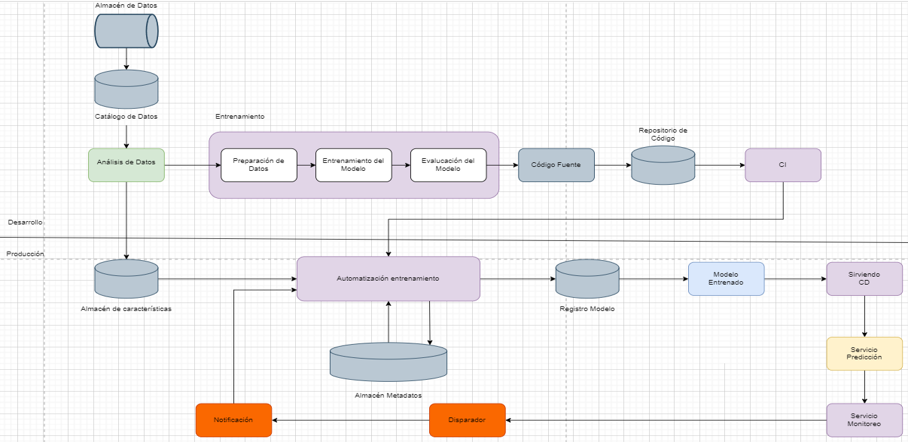
\includegraphics[width=1\textwidth]{resultados/flujoMLOps.png}
\caption*{\footnotesize Fuente: Elaboración Propia}
\label{fig:figuraFlujoMLOps}
\end{figure}

Se observa un proceso que se divide en dos etapas fundamentales: la etapa de desarrollo y la etapa de producción. En la fase de desarrollo, que generalmente se alinea con los objetivos uno y dos, se enfoca en el preprocesamiento de datos, abordando tareas como normalización, escalado de imágenes o redimensionamiento a dimensiones específicas. \newline

Durante esta etapa, se inicia la definición del entrenamiento y evaluación de datos. Con la implementación del MLOps, se introduce el versionado del código, permitiendo el control de cambios y la trazabilidad de la información. Un aspecto destacado es la iniciación del versionado de datos, donde se almacenan características específicas. En el contexto de un modelo de regresión logística, se determinan parámetros críticos como la cantidad de ciclos para el balanceo de datos, el tamaño de la muestra y el porcentaje asignado para las pruebas, cumpliendo con el previamente establecido 20\%. En la fase de producción se identifican los procesos de guardar la información esencial, como los modelos resultantes y sus respectivos desempeños, precisión y otros indicadores, todo centralizado en un sistema de registro de modelos. \newline

Continuando con el flujo del proceso, se registra la información del código fuente, es decir, la ubicación donde se crearon los códigos para la generación del modelo, siendo esta información cargada en una fuente de datos en línea. Este momento marca la viabilidad de realizar la integración continua, que se lleva a cabo mediante la misma herramienta de versionado de código, estableciendo así un flujo de trabajo continuo en el desarrollo del modelo. \newline

La fase de integración continua se realiza a través de la misma herramienta de repositorio de código que respalda el versionado del código. A continuación, se automatiza el proceso de entrenamiento del modelo, descrito en la fase de producción, que contribuye a una automatización progresiva. En este enfoque, el entrenamiento se configura automáticamente en intervalos regulares o después de ciertas tareas específicas, generando de manera continua registros de modelos en desarrollo. \newline

En otras palabras, cada vez que se inicia un entrenamiento, se registra un nuevo modelo, listo para su implementación posterior. Este modelo entrenado se despliega y se expone a través de una API, facilitando el acceso desde diversos dispositivos, ya sea una computadora o un teléfono celular. Además, se crea una aplicación web que permite a los usuarios cargar imágenes simples para realizar predicciones sobre la presencia o ausencia de plagas. \newline

El proceso se complementa con un servicio de monitoreo diseñado para supervisar, registrar y verificar la información de los distintos modelos. Este monitoreo también se utiliza para analizar el rendimiento de los modelos, y en caso de un bajo rendimiento según las métricas establecidas, se activa un mecanismo de notificación. \newline

\newpage

Cuando el sistema detecta un bajo rendimiento, se dispara una notificación, generalmente a través de correo electrónico, que se envía directamente a un científico de datos. Este profesional evalúa la situación y determina los procesos a seguir para modificar y mejorar el rendimiento del modelo. El ciclo de integración continua, entrenamiento automatizado y monitoreo proactivo contribuyen a mantener y mejorar constantemente la eficacia de los modelos en producción. \newline

Un proceso de entrenamiento de un modelo debe ser escalable, colaborativo y reproducible. Los principios, herramientas y técnicas que garantizan que la construcción de modelos sea escalable, colaborativo y reproducible se conoce como MLOps. El MLOps seria llevar un modelo de ML desde su etapa de desarrollo a la etapa de producción y que se encuentre disponible para un usuario final, y a su vez sea confiable y eficiente.

Dentro de las características del MLOps confiable y eficiente se encuentran:

\begin{itemize}
    \item Buenas prácticas para crear código (variables y funciones de métodos adecuados para que se entienda el código elaborado).
    \item Control de versiones (código, datos y modelos de ML).
    \item Pruebas automáticas (sobre el flujo del sistema de ML para evitar fallas en el modelo que es el usado por los usuarios finales).
    \item Reproducibilidad (ayuda a obtener y replicar los mismos resultados con los datos y modelos anteriores).
    \item Documentación (ayuda a entender como fue realizado el código).
    \item Monitoreo (verifica cambios que pasan con el tiempo al modelo).
\end{itemize}

\newpage

A partir de estas características y específicamente después de realizar varias iteraciones para ajustar la parametrización de los modelos, se busca determinar cuál es el modelo óptimo que será implementado en producción. Durante este proceso de búsqueda, se versiona cada uno de los modelos en consideración y se compara su rendimiento para identificar el más eficiente. Cabe señalar que, se llevan a cabo pruebas automáticas en todo el modelo, contribuyendo así a la detección y prevención de posibles fallos en el flujo del modelo para ponerlo en producción. \newline

Las pruebas se realizan al modelo, siempre y cuando este no sea demasiado complejo de reentrenar o validar. En particular, se destaca que es más factible y eficiente entrenar el modelo de regresión logística en comparación con modelos más exigentes computacionalmente, como el modelo Yolo V8. Incluso con el primero, es posible usar la CPU únicamente para obtener un resulto, en contraste, el segundo requiere de la CPU y GPU simultáneamente. \newline

En el contexto de la reproducibilidad, se refiere a la capacidad de tener los datos en un punto específico, lo que significa que se puede rastrear qué datos se utilizaron exactamente para entrenar un modelo en particular. La reproducibilidad es esencial para replicar resultados en diferentes momentos en el tiempo. Este proceso se ve facilitado mediante una documentación que ayuda a comprender las acciones realizadas, especialmente en relación con el código de la solución implementada. La documentación proporciona la transparencia necesaria para entender el enfoque adoptado y los resultados obtenidos en cada fase del proceso.

\newpage

\begin{longtable}{|p{3cm}|p{5cm}|p{6cm}|}
\caption{Flujo de trabajo con MLOps}\\
    \hline
    \textbf{Elementos} & \textbf{Características} & \textbf{Acciones} \\
    \hline
    \endhead
        Análisis de datos & El análisis de datos se refiere al proceso de inspeccionar, limpiar, transformar y modelar datos con el objetivo de descubrir información útil, llegar a conclusiones y respaldar la toma de decisiones. & Durante esta etapa, se aborda la tarea de comprender la naturaleza de los datos, especialmente en el contexto de la identificación de plagas. Se busca discernir la presencia o ausencia de plagas, examinando la estructura y características de los datos. Se destacan acciones específicas, como la identificación de dimensiones desiguales en los datos, donde algunas muestras presentan mayor cantidad de píxeles en el ancho que en la altura. Ante esta diversidad, se afronta el desafío de establecer uniformidad en las dimensiones, asegurando coherencia en el conjunto de datos. \\
        \hline
        Feature Store (almacén de funciones) & Se almacenan las transformaciones que se le han aplicado a los datos, para después entrenar los modelos. & En el modelo de la regresión logística se remueve el fondo de las imágenes y después se redimensionan a un valor indicado de 640 x 640 pixeles. \\
        \hline
        Versionado del código & En donde se guarda todo el código generado, y se sube a internet. & Facilitar una integración adecuada de la solución realizada para los modelos tanto de regresión logística como Yolo V8. \\
        \hline
        Integración continua & Se refiere a la práctica de fusionar y validar regularmente los cambios de código en un repositorio compartido. & Permitir que diferentes miembros de un equipo de trabajo, pueden realizar una integración correcta de los códigos que se van agregando a un repositorio. \\
        \hline
        Versionado del modelo & Permite cambiar entre modelos en tiempo real o monitorear diferentes modelos & Se verifica cómo se van comportando los modelos dependiendo a parámetros que se le vayan cambiando y determinar cuál entre ellos es el mejor y poder después de haberlo identificado colocarlo en producción.  \\
        \hline
        Registro de modelos & Una vez que se ha entrenado un modelo, se almacena en un sistema de registro de modelos junto con sus metadatos. & Selección de parámetros por modelo a registrar, como ciclos de entrenamiento y numero de imágenes a emplear para la regresión logística. Cada una de estos parámetros, junto con el modelo entrenado, es agregado de manera integral al registro del modelo. La práctica de agregar estos metadatos al registro del modelo se realiza de manera continua, generando así versiones sucesivas del modelo a medida que se lleva a cabo el proceso de validación. \\
        \hline
        Model serving & Desplegar el modelo para que pueda ser usado por los usuarios, por medio de API y/o aplicación. & Sea en un computador, en una tablet o en un celular, el acceso al modelo se facilita para cualquier usuario, ya sea un individuo común o incluso un científico de datos. Se desarrolla una API y una aplicación con la finalidad de que el usuario final, pueda observar el comportamiento del modelo. La API y la aplicación permite pasar datos de prueba o datos reales, permitiendo así la validación de la existencia o no de plagas en un aguacate Hass. \\
        \hline
        Monitoreo de modelos & Se deben monitorear los modelos, para detectar cambios en el desempeño o puesta en producción. Esto es debido a que los modelos en producción pueden degradarse con el tiempo por los cambios en los datos de entrada, fallas en el sistema o fallas al momento de la generación del modelo. & Se lleva a cabo una monitorización continua para identificar cualquier cambio que pueda surgir en el rendimiento de un modelo. Este cambio puede manifestarse a través de variaciones en el rendimiento comparándose con una métrica global, así como errores de los servicios. Estas discrepancias pueden originarse por posibles fallas en diversas etapas del proceso. \\
        \hline
        CI / CD & Garantizan que el código se fusione frecuentemente donde se realicen compilaciones y pruebas automatizadas en un repositorio central. & En el proceso de MLOps, implica no solo probar el código, sino los modelos resultantes y desplegar el modelo en una API y/o una aplicación para los usuarios finales. \\
        \hline
        Almacén de metadatos & El registro es fundamental para la reproducibilidad. Se pueden registrar todos los parámetros pasados a un modelo, como las métricas después de evaluarlo o registros del hardware usado. & Se permite el registro de información de los modelos, debido a que es parte esencial para la reproducibilidad. Esto implica la retención de información, específica para el modelo, como los parámetros y las iteraciones realizadas, así como la cantidad de datos empleados durante el proceso de entrenamiento de un modelo, entre otros. Este registro es para garantizar la capacidad de reproducir exactamente las condiciones bajo las cuales se desarrolló un modelo en particular. \\
        \hline
        Almacén de metadatos & El registro es fundamental para la reproducibilidad. Se pueden registrar todos los parámetros pasados a un modelo, como las métricas después de evaluarlo o registros del hardware usado. & Se permite el registro de información de los modelos, debido a que es parte esencial para la reproducibilidad. Esto implica la retención de información, específica para el modelo, como los parámetros y las iteraciones realizadas, así como la cantidad de datos empleados durante el proceso de entrenamiento de un modelo, entre otros. Este registro es para garantizar la capacidad de reproducir exactamente las condiciones bajo las cuales se desarrolló un modelo en particular. \\
    \hline
    \caption*{\footnotesize Fuente: Elaboración propia}
    \label{tab:tabCicloMlops}
\end{longtable}

Profundizando en el ciclo del MLOps, se retoma la referencia previa a la integración continua y despliegue continuo. Estas dos fases trabajan en conjunto para asegurar que el código se fusiona de manera regular y que las implementaciones son compiladas y automatizadas en un repositorio central. La integración continua se centra en fusionar el código con frecuencia, implementando compilaciones automatizadas que son almacenadas en un repositorio central.

\newpage

En cuanto al proceso, no se limita únicamente a probar el código; también implica evaluar los modelos resultantes. Este paso incluye el despliegue del modelo en una aplicación, permitiendo que los usuarios finales consuman los resultados. La entrega continua va más allá, implicando la implementación de cambios en el código en un entorno de pruebas o producción. Esta fase facilita despliegues rápidos para corregir fallos o implementar cambios en un modelo, posibilitando su incorporación en un entorno de producción.

\subsubsection{Las diferentes herramientas que implementan MLOps}

Entre las diversas herramientas disponibles para el MLOps, se pueden clasificar en dos categorías distintas: las sencillas y las complejas. Las herramientas sencillas son particularmente útiles para facilitar el despliegue local, es decir, en un mismo ordenador o un servidor local. Este enfoque es especialmente adecuado para pequeñas empresas o equipos pequeños de investigación, donde varios miembros de un equipo de trabajo pueden acceder desde diferentes computadoras de manera local. Estas herramientas sencillas representan el primer paso para llevar la solución a la fase de despliegue, especialmente en entornos de producción. \newline

Por otro lado, las herramientas complejas están diseñadas para gestionar mayores capacidades de cómputo. Estas pueden configurarse con capacidades específicas, e incluso el sistema puede autoajustarse según el tráfico y los requisitos de almacenamiento, incorporando la funcionalidad conocida como ``On Demand'', donde son capaces de autoescalar según las necesidades del momento. \newline

\newpage

Después de implementar las herramientas sencillas, se puede aprovechar lo creado para desplegar una aplicación. Esta aplicación, inicialmente desarrollada o creada localmente, puede integrarse con uno de los servicios en la nube más comunes y populares. Estos servicios en la nube, como AWS, Azure, GCP, son seleccionados debido a su amplia cuota de mercado y su uso generalizado en la actualidad. Esto permite llevar la aplicación creada localmente a aprovechar las capacidades y escalabilidad que ofrecen los servicios en la nube para su despliegue. \newline

La implementación de un monitoreo completo plantea ciertas consideraciones, especialmente cuando se considera la adopción de herramientas complejas. La complejidad de estas herramientas conlleva un aumento en los costos, ya que se aplican cargos por el conjunto completo de funcionalidades que ofrecen. En comparación, optar por el despliegue local y utilizar solo una fracción de estas herramientas resulta más económico. \newline

Además del aspecto financiero, es crucial tener en cuenta que el uso de herramientas complejas implica una curva de aprendizaje significativa. Se requiere una inversión de tiempo y esfuerzo para adquirir los conocimientos necesarios y comprender cómo manipular eficazmente todo el ciclo del MLOps (ver figura \ref{fig:figuraHerramientasMLOps}). Esta curva de aprendizaje elevada puede representar una desventaja, ya que impone una barrera para aquellos que buscan implementar estas herramientas de manera efectiva. \newline

Se han ido desarrollando muchas herramientas que se pueden utilizar para implementar la metodología de MLOps tanto de acceso libre (open source) o de pago, para usar localmente o desde internet. Y se deben escoger cada una con base a las necesidades del proyecto.

\newpage

\begin{figure}[h]
\centering
\caption{Herramientas que implementan ciclo completo de MLOps}
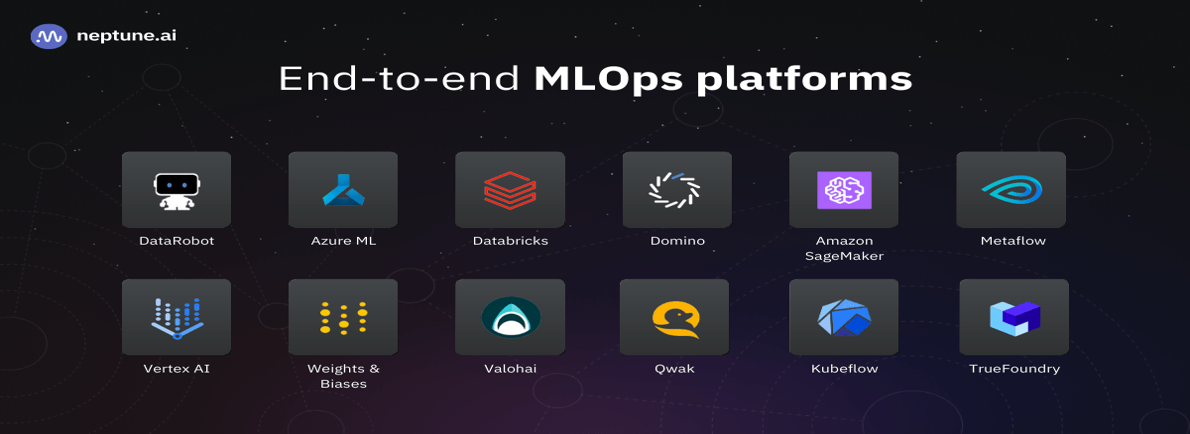
\includegraphics[width=1\textwidth]{resultados/herramientasMLOps.png}
\caption*{\footnotesize Fuente: \cite{neptune2024}}
\label{fig:figuraHerramientasMLOps}
\end{figure}

Dentro de las plataformas descritas en la imagen anterior se encuentra MetaFlow, esta plataforma en sí misma, es una herramienta gratuita, aunque algunas de sus funcionalidades pueden requerir pagos. Por ejemplo, el despliegue en internet podría estar sujeto a tarifas adicionales. Para completar todo el ciclo de vida del MLOps, es necesario considerar diversas herramientas, muchas de las cuales ofrecen características completas o parciales para gestionar eficazmente este ciclo. \newline

Para esta investigación se optó por seleccionar metodologías Open Source y se integraron  con Google Cloud Platform (GCP) para aprovechar características específicas. Aunque GCP es un servicio de pago, se ha utilizado la opción gratuita que proporciona un periodo de 90 días con fines educativos. Antes de que expire este período, es necesario cerrar la cuenta para evitar cargos adicionales. \newline

Como se viene mencionando, cada etapa del ciclo de vida del MLOps se cumple, total o parcialmente, mediante el uso de herramientas específicas (ver figura \ref{fig:figuraHerramientasAlmaAuto}, figura \ref{fig:figuraHerramientasAnaRepo}, figura \ref{fig:figuraHerramientasRegModDatos} e figura \ref{fig:figuraHerramientasDespApiApp}). Este enfoque garantiza una implementación efectiva y personalizada del ciclo de vida del MLOps, adaptándolo a las necesidades y requisitos específicos del proyecto.

\newpage

\begin{figure}[h]
\centering
\caption{Herramientas para almacenamiento y automatización de procesos}
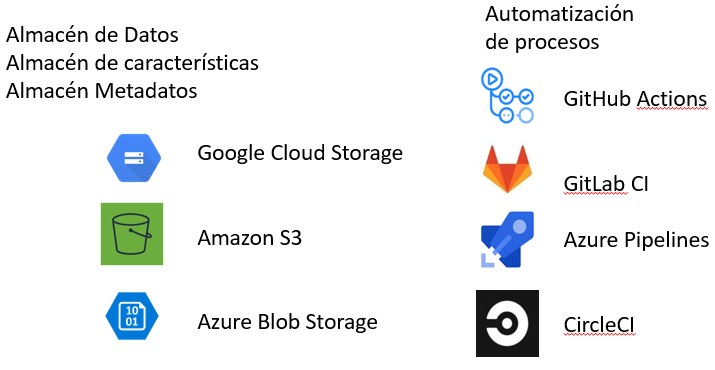
\includegraphics[width=1\textwidth]{resultados/herramientasAlmaAuto.png}
\caption*{\footnotesize Fuente: Elaboración propia}
\label{fig:figuraHerramientasAlmaAuto}
\end{figure}

Para esta implementación de MLOps se utilizó Jupyter, como se viene describiendo desde el objetivo 1. En cuanto al repositorio de código es en GitHub, que es una plataforma líder en el desarrollo colaborativo de software que proporciona servicios de alojamiento de repositorios Git, permitiendo a los miembros de un equipo trabajar juntos en proyectos, gestionar versiones de código y facilitar la colaboración distribuida.

\newpage

\begin{figure}[h]
\centering
\caption{Herramientas de análisis de datos y repositorio de código}
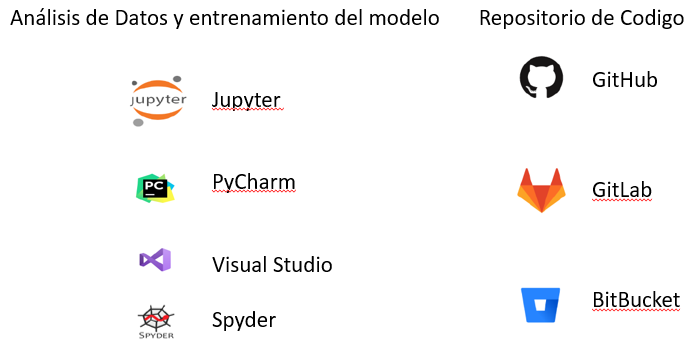
\includegraphics[width=1\textwidth]{resultados/herramientasAnaRepo.png}
\caption*{\footnotesize Fuente: Elaboración propia}
\label{fig:figuraHerramientasAnaRepo}
\end{figure}

\newpage

\begin{figure}[h]
\centering
\caption{Herramientas de registro de modelo, versionado del modelo y versionado de datos}
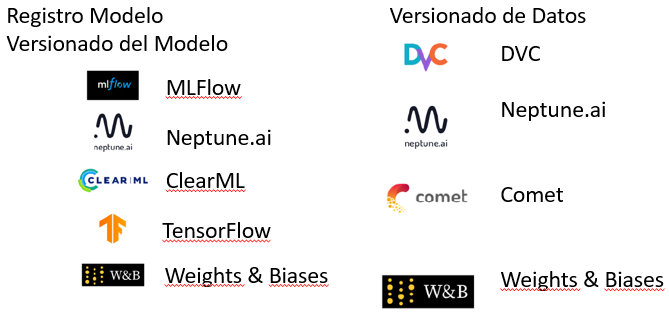
\includegraphics[width=0.7\textwidth]{resultados/herramientasRegModDatos.png}
\caption*{\footnotesize Fuente: Elaboración propia}
\label{fig:figuraHerramientasRegModDatos}
\end{figure}

\begin{figure}[h]
\centering
\caption{Herramientas para Construcción de API y Construcción de aplicación Web}
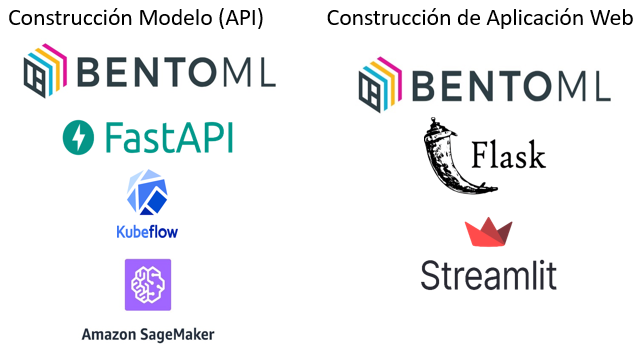
\includegraphics[width=0.6\textwidth]{resultados/herramientasDespApiApp.png}
\caption*{\footnotesize Fuente: Elaboración propia}
\label{fig:figuraHerramientasDespApiApp}
\end{figure}

\newpage

\begin{figure}[h]
\centering
\caption{Herramientas de Feature Store y Monitoreo del Modelo}
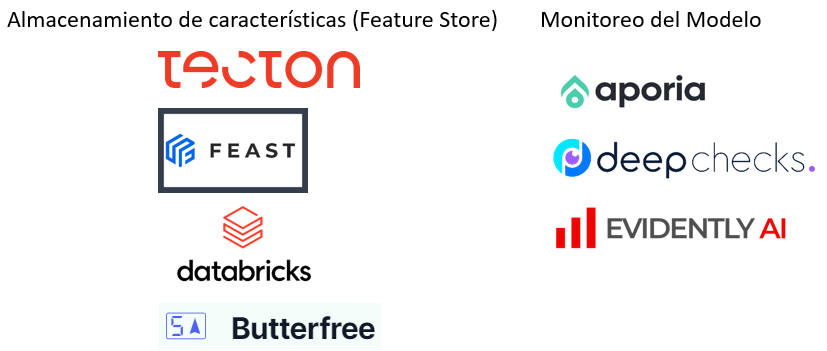
\includegraphics[width=0.9\textwidth]{resultados/herramientasFeaMon.png}
\caption*{\footnotesize Fuente: Elaboración propia}
\label{fig:figuraHerramientasFeaMon}
\end{figure}

\begin{figure}[h]
\centering
\caption{Herramientas utilizadas en el proyecto de MLOps para plagas en aguacate Hass}
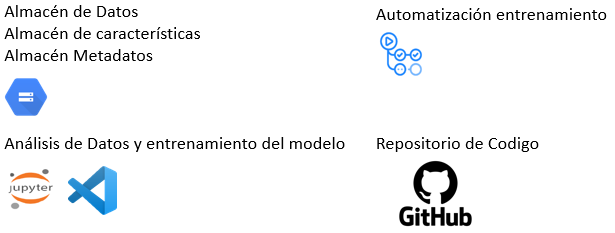
\includegraphics[width=0.7\textwidth]{resultados/herramientasAlmAutoAnaRep.png}
\caption*{\footnotesize Fuente: Elaboración propia}
\label{fig:figuraHerramientasAlmAutoAnaRep}
\end{figure}

\newpage

Las herramientas seleccionadas, como se mencionó una de ellas es Google Cloud Storage, elegida por su acceso gratuito durante 90 días, lo que permite manipular eficazmente este almacenamiento. Además, Google Cloud ofrece un crédito de alrededor de \$300 para utilizar diversas funciones de Google, lo cual resulta beneficioso para el análisis de datos. \newline

Otra herramienta clave es Visual Studio Code, que desempeñó un papel esencial en las transformaciones mencionadas. Fue especialmente útil para la transformación de los cuadernos de Jupyter a Python, proporcionando una interfaz intuitiva para manipular el código directamente en formato Python. Esto facilitó la gestión del código en un repositorio utilizando Git, donde se lleva a cabo el versionado de todas las partes del código y todo lo realizado en el desarrollo.

\newpage

\begin{figure}[h]
\centering
\caption{Herramientas utilizadas en el proyecto de MLOps para plagas en aguacate Hass}
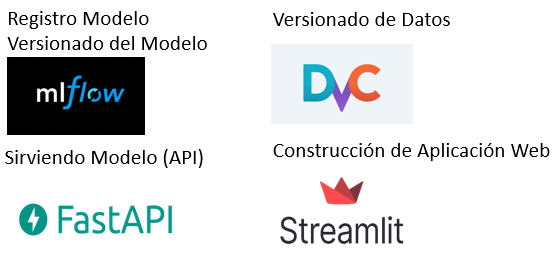
\includegraphics[width=0.7\textwidth]{resultados/herramientasRegVerCons.png}
\caption*{\footnotesize Fuente: Elaboración propia}
\label{fig:figuraHerramientasRegVerCons}
\end{figure}

Para el registro de modelos, se optó por MLFlow, una herramienta elegida por su eficacia en la gestión de versiones de modelos. En el ámbito del versionado de datos, se seleccionó la herramienta DVC, que facilita el almacenamiento de los datos por versiones. Para la construcción de aplicaciones web, se utilizó Streamlit. Para la implementación de la API, tanto local como remotamente, se empleó FastAPI. Es importante señalar que esta parte del proyecto, aunque extensa, es una extensión de la actividad 2 del objetivo tres, que implica la identificación de las herramientas empleadas para desarrollar la metodología MLOps en el proyecto.

\newpage

\begin{figure}[h]
\centering
\caption{Herramientas utilizadas en el proyecto de MLOps para plagas en aguacate Hass}
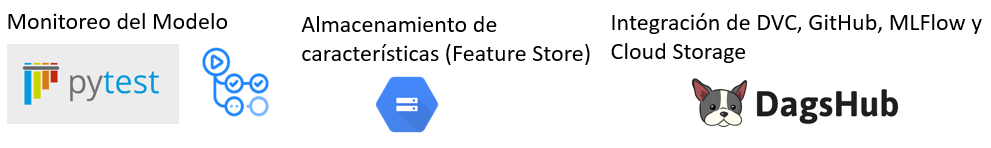
\includegraphics[width=0.7\textwidth]{resultados/herramientasMonAlmInt.png}
\caption*{\footnotesize Fuente: Elaboración propia}
\label{fig:figuraHerramientasMonAlmInt}
\end{figure}

En lo que respecta al monitoreo del modelo, se eligió realizar pruebas con Pytest, una dependencia de Python que evalúa el código y ejecuta pruebas. Este proceso de evaluación se lleva a cabo de manera programada a diario a las 4 de la mañana utilizando GitHub Actions, una herramienta de automatización de procesos. \newline

La elección del horario específico, las 4 de la mañana, se estableció para automatizar la ejecución de tareas en un momento menos propenso a la manipulación activa de modelos, especialmente por parte de los científicos de datos. No obstante, este horario podría ajustarse según necesidades y criterios específicos. \newline

En cuanto al almacenamiento de características, se utilizó Google Cloud Storage, empleando sus capacidades para almacenar las transformaciones aplicadas a las imágenes en el modelo de regresión logística. Cabe mencionar que, aunque se optó por este modelo para implementar la metodología MLOps debido a su menor consumo de recursos computacionales y tiempos de respuesta más rápidos en comparación con el modelo Yolo, esta metodología también se podría adaptar para Yolo según los requisitos específicos del modelo. \newline

Estas herramientas, cuidadosamente seleccionadas, ofrecieron una solución integral que abarcó desde el almacenamiento y análisis de datos hasta la gestión efectiva del código, de los datos, de los modelos y sus versiones, contribuyendo así al éxito del proyecto en el ámbito de la ingeniería de software.

\newpage

\subsubsection{Integración con herramientas MLOps}

Después de haber identificado las herramientas utilizadas para implementar MLOps. La sección se centra en el uso de estas herramientas y destaca el código disponible en un enlace proporcionado, organizado en una estructura específica de carpetas basada en una plantilla de ciencia de datos de cookiecutter\footnote{La plantilla se encuentra en el siguiente enlace de acceso público en GitHub \href{https://github.com/khuyentran1401/data-science-template/tree/dvc-pip}{aquí}.}, la cual es una dependencia de Python. El enlace a continuación proporciona acceso al código completo del proyecto, organizado de manera estructurada en carpetas con GitHub\footnote{Las carpetas y el código se encuentran en el siguiente enlace de acceso público en GitHub \href{https://github.com/juferoto/mlops_project}{aquí}.}.

\begin{figure}[h]
\centering
\caption{Estructura de las carpetas para el proyecto}
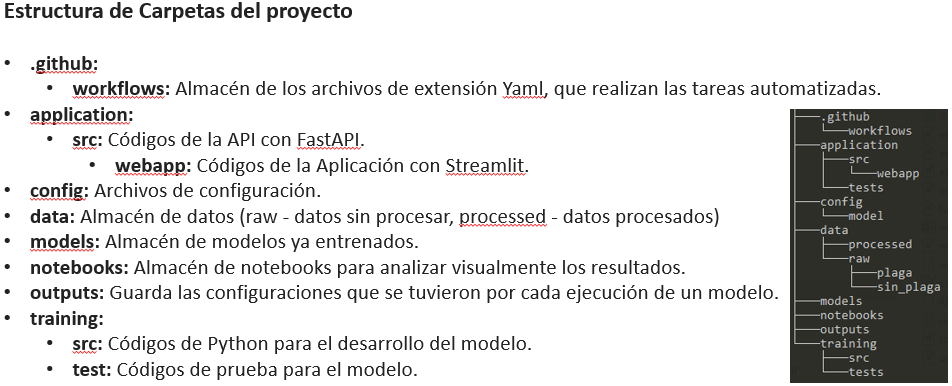
\includegraphics[width=1\textwidth]{resultados/estructuraCarpetas.png}
\caption*{\footnotesize Fuente: Elaboración propia}
\label{fig:figuraEstructuraCarpetas}
\end{figure}

La estructura de carpetas utilizada es esencial para comprender la lógica detrás de la implementación. Uno de los componentes de esta estructura es el ``workflows'', que almacena los archivos con extensiones Yaml y actúa como la base de las tareas automatizadas. Este punto será abordado de manera más detallada en el objetivo 4. Este enfoque en la organización y el propósito de las carpetas proporciona una visión clara de la implementación subyacente.

\newpage

Para realizar la ejecución local y obtener la estructura completa de carpetas desde el enlace proporcionado, se sigue un proceso que implica la clonación del repositorio desde GitHub. Una vez obtenida la información localmente, el código disponible puede ejecutarse para aquellos que lo necesiten. Todas las dependencias necesarias para el funcionamiento sin problemas del proyecto localmente están detalladas a continuación:


\begin{figure}[h]
\centering
\caption{Dependencias para trabajar con el proyecto localmente}
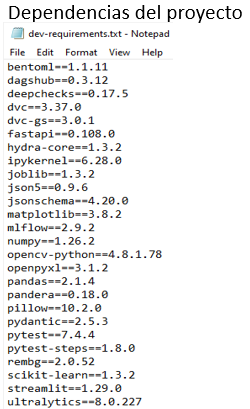
\includegraphics[width=0.5\textwidth]{resultados/dependenciasLocal.png}
\caption*{\footnotesize Fuente: Elaboración propia}
\label{fig:figuraDependenciasLocal}
\end{figure}

\newpage

Las dependencias del proyecto para trabajar de forma local se encuentran en la raíz del proyecto, en un archivo llamado dev-requirements.txt. Para instalar las diferentes dependencias seria con el comando: 
\begin{verbatim}
pip install -r dev-requirements.txt
\end{verbatim}

Cuando se clona el proyecto, se obtienen todos los archivos y carpetas en la ubicación local deseada. Una vez completada la clonación, se puede acceder a la estructura completa del proyecto. Este proyecto ha sido diseñado considerando todas las dependencias necesarias para su ejecución. \newline

En cuanto a la estructura de carpetas, se destaca la carpeta ``models'', que desempeña un papel crucial en el almacenamiento del modelo entrenado. En este contexto, el modelo de regresión logística, se almacena en formato “joblib”, una dependencia de Python diseñada para guardar modelos de Machine Learning de manera eficiente, que facilita su obtención y reproducibilidad. \newline

Adicionalmente, se tiene la carpeta ``notebooks'', la cual contiene los códigos asociados del modelo de regresión logística mencionado anteriormente en formato jpynb de Jupyter Notebook. En este sentido, los mismos códigos utilizados para el objetivo dos del proyecto se encuentran aquí, lo que facilita la revisión y comprensión de las implementaciones.


\begin{figure}[h]
\centering
\caption{Estructura de carpeta models y notebooks}
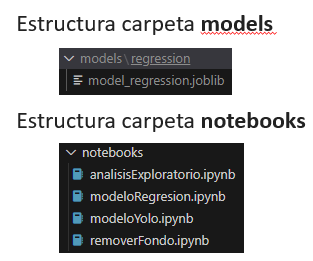
\includegraphics[width=0.8\textwidth]{resultados/estructuraCarModNote.png}
\caption*{\footnotesize Fuente: Elaboración propia}
\label{fig:figuraEstructuraCarModNote}
\end{figure}

\newpage

Cabe resaltar que estos códigos no solo representan lo realizado del modelo de regresión logística, sino que también abarcan los procedimientos aplicados en la implementación del modelo Yolo V8. La inclusión de ambas implementaciones se encuentra en la carpeta ``notebooks'' ofreciendo una visión completa y organizada de las soluciones realizadas, permitiendo una fácil referencia y reproducción de los procesos aplicados. \newline

En pos de simplificar y preservar la integridad de las configuraciones durante el entrenamiento o evaluación de un modelo, se implementó una estrategia que evita la manipulación directa de los valores dentro del código. Para lograr esto, se incorporó una dependencia adicional llamada Hydra, la cual facilita la gestión de configuraciones al externalizarlas en archivos dedicados.

\newpage

En lugar de codificar valores directamente, se optó por utilizar archivos de configuración, aprovechando la funcionalidad proporcionada por Hydra. Esta herramienta permite centralizar todas las configuraciones en un archivo específico, que contiene los parámetros que definen la configuración para la ejecución de un programa. Estos archivos de configuración adoptan el formato YAML, proporcionando una estructura clara y legible, la adopción de archivos de configuración no solo mejora la legibilidad del código al eliminar valores directos, sino que también facilita la adaptabilidad del programa a diferentes contextos y escenarios. \newline

Otro aspecto es que, con Hydra, cada vez que se evalúa un modelo, las configuraciones se guardan automáticamente en una carpeta designada llamada ``outputs''. En esta carpeta, cada ejecución del modelo genera automáticamente un subdirectorio con la fecha, hora, minutos y segundos precisos en los que se llevó a cabo. Este enfoque asegura un registro detallado de las configuraciones utilizadas en cada ejecución, lo que no solo facilita la reproducibilidad, sino que también permite un seguimiento de los parámetros específicos utilizados en diferentes ejecuciones.

\begin{figure}[h]
\centering
\caption{Estructura carpeta outputs}
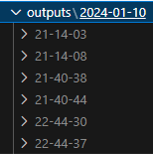
\includegraphics[width=0.4\textwidth]{resultados/carpetaOutputs.png}
\caption*{\footnotesize Fuente: Elaboración propia}
\label{fig:figuraEstructuraCarpetaOutputs}
\end{figure}

\newpage

Este enfoque ofrece una trazabilidad exhaustiva, beneficiando a aquellos que requieren información detallada sobre las ejecuciones del modelo, y también contribuye al registro y versionado de los modelos. Cada ejecución crea un marcador temporal, proporcionando una forma sistemática y organizada de rastrear las diferentes versiones del modelo. Además, se extiende al versionado de los datos, lo que añade un nivel adicional de control y seguimiento en cada ejecución de un modelo. \newline

En el archivo main.yml, se guardan todas las configuraciones que se tienen para el proyecto, como las variables al seleccionar el modelo por defecto a trabajar, que en este caso es el modelo de regresión logística. Como también, la ruta en donde se encuentran ubicadas las imágenes procesadas de la información del cultivo del aguacate Hass, las cuales pueden variar en términos de tener o no tener fondo. Todas estas imágenes se almacenan en la carpeta “data/raw” y se guardan los dos tipos mencionados en el objetivo uno: las imágenes con plaga y las imágenes sin plaga.

\begin{figure}[h]
\centering
\caption{Configuraciones del archivo main.yml y del archivo model1.yml}
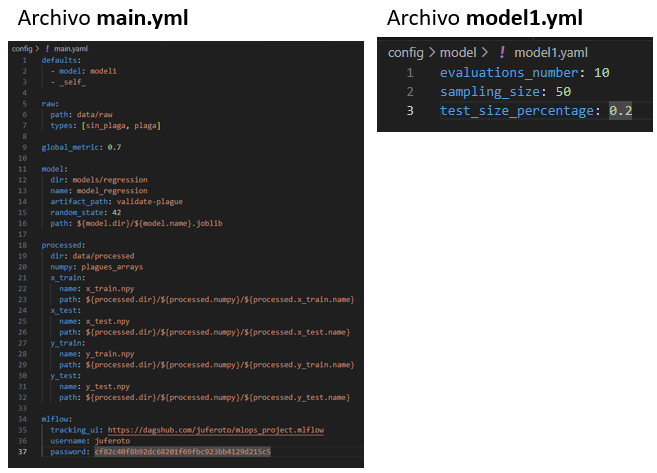
\includegraphics[width=0.7\textwidth]{resultados/configuracionesMain.png}
\caption*{\footnotesize Fuente: Elaboración propia}
\label{fig:figuraConfiguracionesMain}
\end{figure}

\newpage

Es en esta sección donde se define la ubicación específica para almacenar el modelo de regresión. La carpeta designada para este propósito es la carpeta ``models'', y se asigna un nombre único a dicho modelo. El ``artifact path'' es un componente manejado internamente por la herramienta MLFlow, para identificar el espacio de trabajo en donde se van almacenar los distintos modelos. \newline

Además, se configura el ``random state'' para la división de conjuntos de entrenamiento y prueba. Aunque esta división se realiza de manera aleatoria, se garantiza que, aunque sea de manera aleatoria, la semilla (random state) permanezca constante. Este enfoque asegura que, al ejecutar el código en diferentes maquinas locales o remotas, se obtenga consistentemente la misma información en términos de conjuntos de datos de entrenamiento y prueba. \newline

En la ruta especificada ``data/processed'', es donde se almacena la información ya procesada, es decir, las transformaciones que se realizan al modelo, como la redimensión de las imágenes, la normalización y la eliminación de fondos de las imágenes. \newline

Durante este proceso, la información se redimensiona, normaliza y se eliminan los fondos de las imágenes, acciones fundamentales en la solución del modelo de regresión lineal. Además, se establecen diferentes conjuntos de entrenamiento y pruebas utilizando las variables disponibles en el archivo ``model1''. \newline

Además, se tienen las configuraciones de acceso de la herramienta MLFlow para realizar el versionado de datos. La función específica de esta configuración se explicará detalladamente en el objetivo cuatro. En resumen, MLFlow desempeña un papel crucial en el seguimiento y versionado de los datos, proporcionando un registro detallado de las diferentes iteraciones y cambios realizados durante el proceso de entrenamiento de un modelo. La configuración detallada no solo garantiza la consistencia en la preparación de datos y la separación de conjuntos, sino que también establece las bases para el seguimiento exhaustivo del versionado de datos a lo largo del proyecto.

\newpage

Como se mencionó anteriormente, fue necesario reestructurar por completo el modelo de regresión logística, trasladándolo desde cuadernos de Jupyter a extensión Python. Esta transformación se llevó a cabo con el objetivo de simplificar el proceso, especialmente para poder llevar a cabo la implementación de tareas automatizadas. La reorganización del código implicó la división en archivos separados, cada uno destinado a cumplir una función específica. Los archivos son: \newline

\begin{itemize}
    \item \textbf{evaluate\_model.py}: Aquí se tiene una función que evalúa el modelo que se acaba de generar después de haberlo procesado y entrenado. Se hace con los conjuntos de prueba generados de la función que está en el archivo process.py (ver figura \ref{fig:figuraCodEvaModel}).
    \item \textbf{helper.py}: Aquí se tiene una función que se crea con el propósito de loguear información para la herramienta de registro de modelos MLFlow (ver figura \ref{fig:figuraCodHelper}).
    \item \textbf{main.py}: Aquí se tiene una función encargada de ejecutar paso a paso todo el proceso de generación del modelo de ML (procesamiento de las imágenes, entrenar y evaluar el modelo) (ver figura \ref{fig:figuraCodMain}).
    \item \textbf{preprocessor.py}: Esta es una clase auxiliar que se contiene las funciones para remover el fondo de las imágenes del aguacate y para cambiar el tamaño de las imágenes (normalizar las imágenes) a valores entre 640 X 640 (ver figura \ref{fig:figuraCodPreprocessor}).
    \item \textbf{process.py}: Aquí se tiene una función que llama a la clase auxiliar preprocessor.py para realizar el procesamiento de las imágenes y así generar los diferentes conjuntos de entrenamiento y pruebas que se van a usar para entrenar el modelo (ver figura \ref{fig:figuraCodProcess}).
    \item \textbf{train\_model.py}: Aquí se tiene una función que se encarga de entrenar el modelo, con los conjuntos de entrenamiento generados de la función que esta en el archivo process.py (ver figura \ref{fig:figuraCodTrainModel}).
\end{itemize}

\newpage

\begin{figure}[h]
\centering
\caption{Código del archivo evaluate\_model.py}
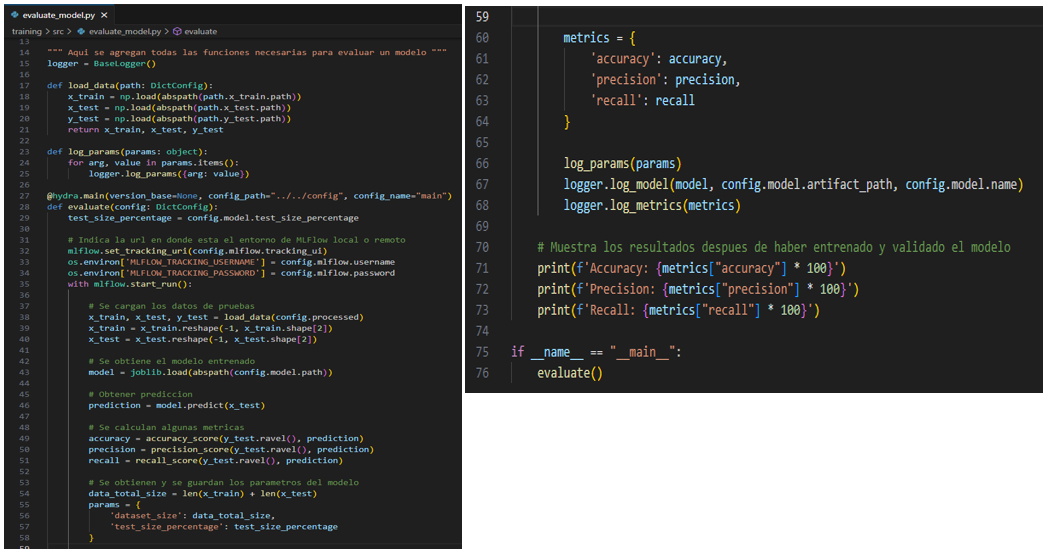
\includegraphics[width=1\textwidth]{resultados/codEvaModel.png}
\caption*{\footnotesize Fuente: Elaboración propia}
\label{fig:figuraCodEvaModel}
\end{figure}

\newpage

\begin{figure}[h]
\centering
\caption{Código del archivo helper.py}
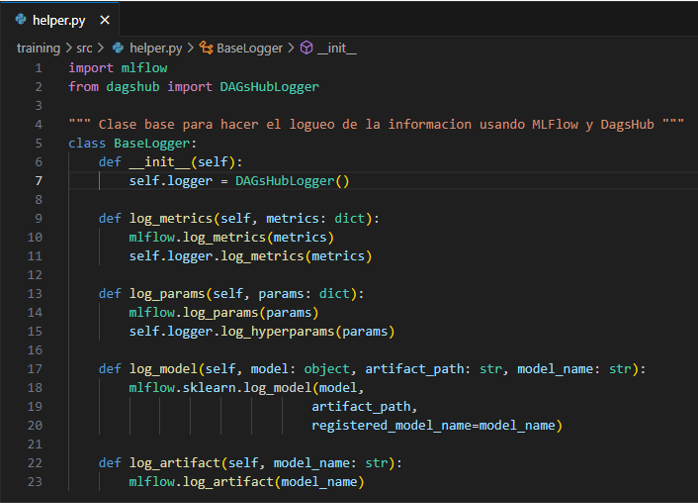
\includegraphics[width=1\textwidth]{resultados/codHelper.png}
\caption*{\footnotesize Fuente: Elaboración propia}
\label{fig:figuraCodHelper}
\end{figure}

\newpage

\begin{figure}[h]
\centering
\caption{Código del archivo main.py}
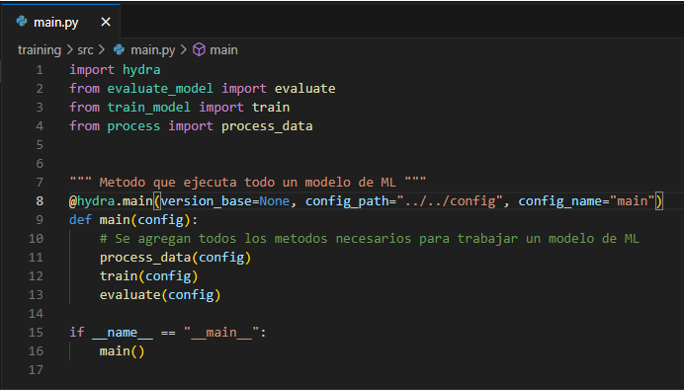
\includegraphics[width=1\textwidth]{resultados/codMain.png}
\caption*{\footnotesize Fuente: Elaboración propia}
\label{fig:figuraCodMain}
\end{figure}

\newpage

\begin{figure}[h]
\centering
\caption{Código del archivo preprocessor.py}
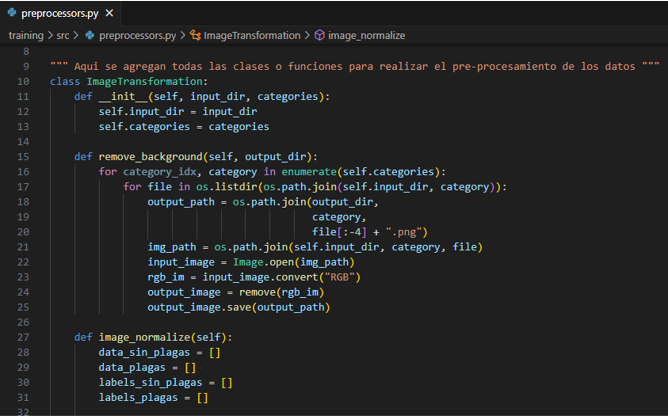
\includegraphics[width=0.7\textwidth]{resultados/codPreprocessor.png}
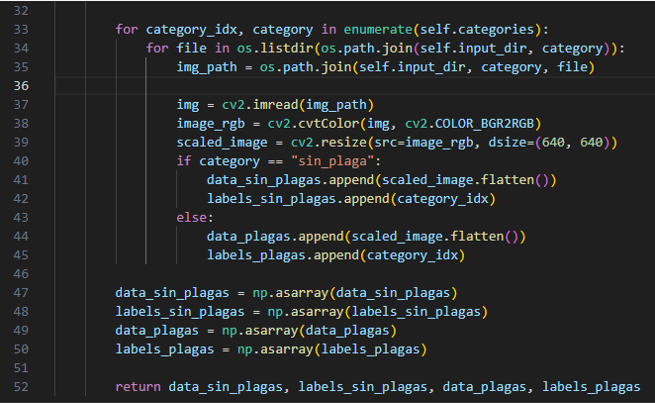
\includegraphics[width=0.6\textwidth]{resultados/codPreprocessor2.png}
\caption*{\footnotesize Fuente: Elaboración propia}
\label{fig:figuraCodPreprocessor}
\end{figure}

\newpage

\begin{figure}[h]
\centering
\caption{Código del archivo process.py}
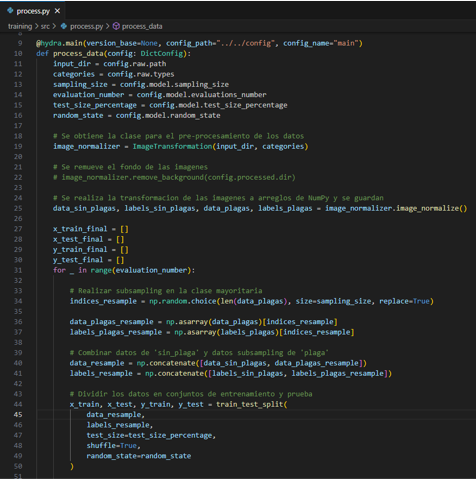
\includegraphics[width=0.6\textwidth]{resultados/codProcess.png}
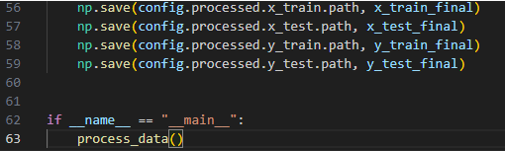
\includegraphics[width=0.6\textwidth]{resultados/codProcess2.png}
\caption*{\footnotesize Fuente: Elaboración propia}
\label{fig:figuraCodProcess}
\end{figure}

\newpage

\begin{figure}[h]
\centering
\caption{Código del archivo train\_model.py}
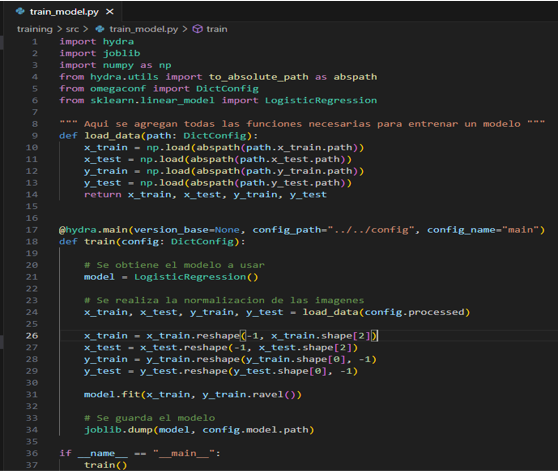
\includegraphics[width=1\textwidth]{resultados/codTrainModel.png}
\caption*{\footnotesize Fuente: Elaboración propia}
\label{fig:figuraCodTrainModel}
\end{figure}

Para entrenar un modelo, se puede realizar mediante la línea de comandos utilizando el siguiente comando en Python: 
\begin{verbatim}
python training\src\main.py
\end{verbatim}

\newpage

Este comando dirige la ejecución al archivo principal main.py ubicado en el directorio `training', iniciando el paso a paso de las operaciones correspondientes, para generar un modelo de regresión logística. Este proceso abarca desde el procesamiento de imágenes hasta el entrenamiento y la evaluación del modelo. \newline

Adicionalmente, durante el proceso se almacenan las métricas resultantes del modelo recién entrenado. Junto con estas métricas, se guarda otra información relevante, como los parámetros utilizados en el modelo. En este caso, se registra el número de evaluaciones, el porcentaje de la prueba y el tamaño del conjunto de datos. Todos estos detalles se conservan para facilitar el registro del modelo utilizando la herramienta de MLFlow, como se mencionó anteriormente.

En relación a como se versiona el código, se realiza por medio de GitHub, la cual es una plataforma web que proporciona servicios para el control de versiones y la colaboración en el desarrollo de software. Algunas características clave y conceptos asociados con GitHub son:

\begin{itemize}
    \item \textbf{Repositorios}: Un repositorio es un espacio donde se almacenan los archivos de un proyecto, junto con la información de seguimiento de versiones. Cada proyecto en GitHub se guarda en un repositorio.
    \item \textbf{Control de Versiones}: GitHub utiliza Git, un sistema de control de versiones distribuido. Esto significa que cada desarrollador o miembro de un equipo, que trabaja en un proyecto tiene una copia completa del historial de cambios del proyecto en su máquina local. Git permite rastrear cambios, fusionar contribuciones y revertir a versiones anteriores del código.
\end{itemize}

\newpage

\begin{figure}[h]
\centering
\caption{Herramienta para versionado de código - GitHub}
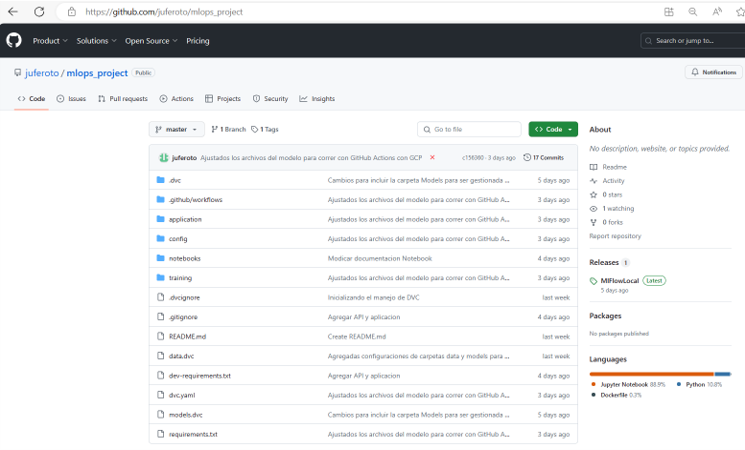
\includegraphics[width=1\textwidth]{resultados/herramientaVerCod.png}
\caption*{\footnotesize Fuente: Elaboración propia}
\label{fig:figuraHerramientaVerCod}
\end{figure}

Ahora, en relación a como se versiona el modelo de regresión logística, pasamos a la herramienta MLOps que estamos aplicando, y esta es MLFlow. Esta es la herramienta elegida para versionar modelos y realizar trazabilidad de experimentos, así como para el registro de modelos. MLFlow es integral para el desarrollo y la gestión de proyectos de aprendizaje automático, facilitando el seguimiento, la reproducción y el registro, así como la trazabilidad de los experimentos. Ofrece una solución unificada que abarca todo el ciclo del MLOps. \newline

Sin embargo, es importante destacar que algunas funcionalidades de MLFlow son de pago. Por esta razón, únicamente estamos utilizando la parte gratuita de ML Flow, específicamente la que se enfoca en el registro de modelos y trazabilidad de experimentos. Estas características permiten almacenar y validar los modelos localmente o incluso en la nube, integrándose si se requiere con otras herramientas.

\newpage

\begin{figure}[h]
\centering
\caption{Herramienta para versionar modelos y trazabilidad de experimentos - MLFlow}
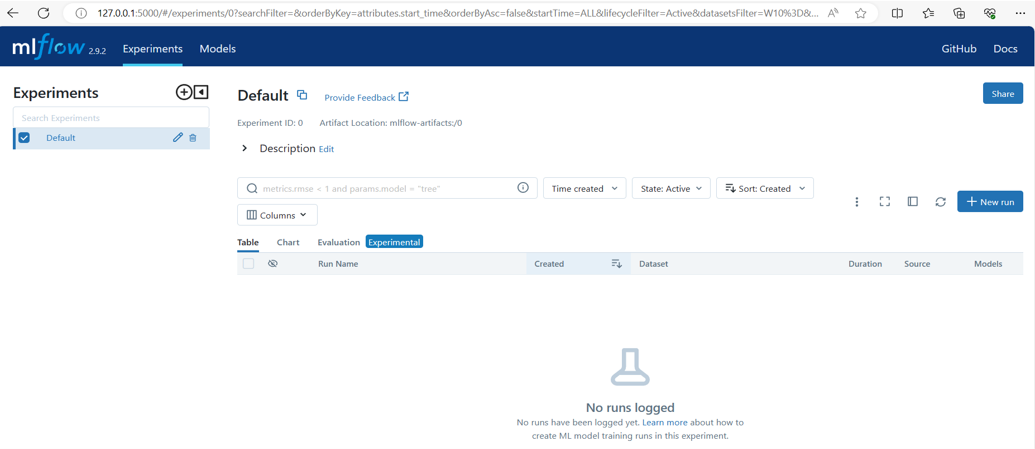
\includegraphics[width=1\textwidth]{resultados/herramientaMlflow.png}
\caption*{\footnotesize Fuente: Elaboración propia}
\label{fig:figuraHerramientaMlflow}
\end{figure}

Esta es la interfaz de MLFlow, donde se presentan de manera clara y organizada cada uno de los experimentos que están en ejecución. Además, se exhiben los modelos que han sido registrados. En un vídeo posterior, detallaré cómo funciona esta herramienta, mostrando paso a paso su operatividad y funcionalidades. \newline

Todas las configuraciones y modelos pueden almacenarse en una máquina o servidor local. Más adelante, en el objetivo cuatro, exploraremos la posibilidad de integrar el MLFlow con una herramienta por internet. Por el momento, se ha optado por la solución local, donde todos los modelos, configuraciones y datos se guardan de manera local. \newline

Con la integración de las herramientas seleccionadas para la metodología MLOps, se cuenta con la presencia de DVC, una herramienta que simplifica la gestión de versiones en proyectos de ciencia de datos y aprendizaje automático. DVC proporciona un control de versiones específico para datos, lo que facilita la colaboración, garantiza la reproducibilidad y favorece la integración con otras herramientas de machine learning.

\newpage

Esta herramienta al permite el versionado de datos, es decir, la capacidad de transitar de un punto a otro, es especialmente útil cuando se ejecuta un código o un modelo. DVC posibilita conocer exactamente cuáles fueron los datos específicos utilizados en una ejecución particular. Así, al ejecutar un modelo y utilizar la versión de datos con DVC, es posible obtener una visión precisa de los datos involucrados en esa ejecución específica.

\begin{figure}[h]
\centering
\caption{Estructura de la carpeta ``data'' del proyecto}
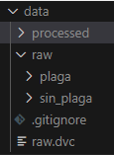
\includegraphics[width=0.4\textwidth]{resultados/estructuraDatos.png}
\caption*{\footnotesize Fuente: Elaboración propia}
\label{fig:figuraEstructuraDatos}
\end{figure}

Para este proyecto en particular, se implementó la siguiente estructura de carpetas para gestionar los datos. En la carpeta ``data’’, se encuentra el subdirectorio ``raw’’, que alberga todos los datos procesados o sin procesar, clasificados en carpetas clave como ``sin plaga’’ y ``con plaga‘’.

\newpage

En la sección ``processed’’, como se detalla en el archivo de configuraciones ``main.yml’’, se encuentran los valores ya procesados y separados en conjuntos de entrenamiento y pruebas. Esta configuración es esencial para la gestión eficiente de DVC. \newline

La estructura de archivos utilizada para el control de versiones de datos se presenta como un ejemplo en pantalla. Automáticamente, al agregar versionado a la carpeta ``raw’’, se genera un archivo como el que se muestra aquí (ver figura \ref{fig:figuraEstructuraArchivoRaw}), el cual es esencial para el versionado de datos con DVC. Este proceso garantiza la trazabilidad y el control de versiones de los datos que se requieren para la ejecución de un modelo.

\begin{figure}[h]
\centering
\caption{Estructura del archivo para realizar control de versiónes de los datos a la carpeta ``data/raw''}
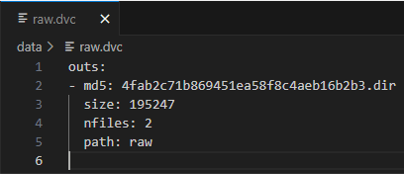
\includegraphics[width=1\textwidth]{resultados/estructuraArchivoRaw.png}
\caption*{\footnotesize Fuente: Elaboración propia}
\label{fig:figuraEstructuraArchivoRaw}
\end{figure}

\newpage

La herramienta DVC, se utiliza comúnmente para registrar el estado de los datos, es decir, en qué punto se encuentran los datos. Estos datos pueden transitar por diferentes estados a lo largo de las diversas etapas del proceso para generar un modelo de regresión logística (ver figura \ref{fig:figuraEstructuraDatosDvc}).

\begin{figure}[h]
\centering
\caption{Estructura de archivos de los datos del proyecto con DVC}
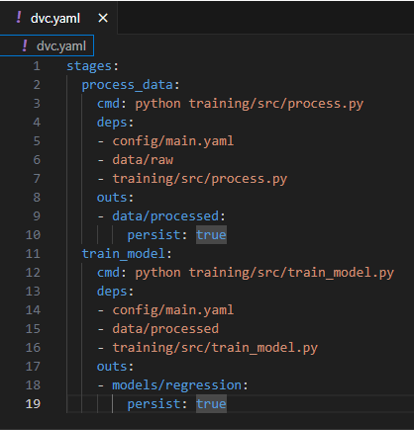
\includegraphics[width=0.8\textwidth]{resultados/estructuraDatosDvc.png}
\caption*{\footnotesize Fuente: Elaboración propia}
\label{fig:figuraEstructuraDatosDvc}
\end{figure}

\newpage

En el contexto de esta investigación, el procedimiento sigue varias etapas. Por ejemplo, existe una etapa en la que los datos se encuentran sin procesar. Luego, se pasa a una etapa donde los datos son procesados y se almacenan en su estado modificado. Posteriormente, se avanza a la etapa de entrenamiento del modelo, y después de completar esta fase, se obtiene un modelo ya entrenado. Por lo tanto, la herramienta DVC permite gestionar eficazmente los diferentes estados de los datos a medida que avanzan a través de las distintas etapas del proceso. \newline

La estructura que se presenta aquí (ver figura \ref{fig:figuraEstadoDatos}) es extraída directamente de la herramienta DagsHub que será detallada en el objetivo cuatro. Esta herramienta integra tanto MLFlow para el versionado de modelos, DVC para el versionado de datos y GitHub para el versionado de código.

\begin{figure}[h]
\centering
\caption{Estado de los datos del proyecto con DVC}
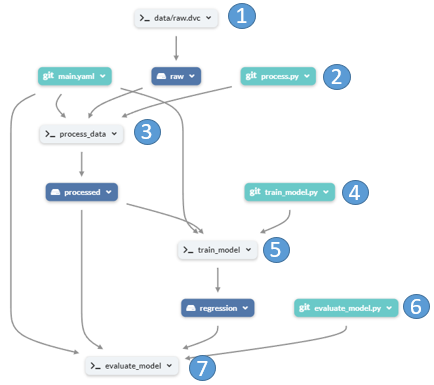
\includegraphics[width=0.7\textwidth]{resultados/estadoDatos.png}
\caption*{\footnotesize Fuente: Elaboración propia}
\label{fig:figuraEstadoDatos}
\end{figure}

\newpage

Estas son las seis etapas de los datos que se están manejando:

\begin{enumerate}
    \item Estado inicial de los datos (datos sin procesar).
    \item Carpeta donde se ubican los datos, archivo de configuración y script para procesar los datos.
    \item Estado que se va a realizar para el proceso de los datos (process\_data).
    \item Carpeta donde se guardan los datos ya procesados y se separan el conjunto de entrenamiento y prueba. También está el script para entrenar el modelo.
    \item Estado que se va a realizar para el entrenamiento del modelo (train\_model).
    \item Carpeta donde se guarda el modelo.
    \item Estado que se va a realizar para la evaluación del modelo (evaluate\_model).
\end{enumerate}

La otra herramienta que es utilizada para la creación de API es FastAPI, la cual es un marco web moderno y rápido para desarrolladores que desean construir APIs rápidas, seguras y bien documentadas con Python\footnote{El código que genera la API se encuentra en el siguiente enlace en GitHub \href{https://github.com/juferoto/mlops_project/tree/master/application/src}{aquí},}. Su enfoque basado en tipos y su compatibilidad con estándares modernos hacen que el desarrollo de APIs sea una tarea eficiente y robusta.

\newpage

\begin{figure}[h]
\centering
\caption{Estructura de la carpeta de la API del proyecto}
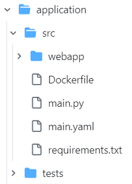
\includegraphics[width=0.3\textwidth]{resultados/estructuraCarpetaAPI.png}
\caption*{\footnotesize Fuente: Elaboración propia}
\label{fig:figuraEstructuraCarpetaAPI}
\end{figure}

Aquí se presenta la estructura de carpetas de la API del proyecto. El archivo Docker, en particular, forma parte del objetivo 4. El código empleado para generar la API está contenido en el archivo ``main.py’’. En este código, se expone un método HTTP - GET que sirve para obtener una respuesta después de que un usuario suba una imagen, para validar contra el modelo seleccionado para ser usado en la API.

\newpage

\begin{figure}[h]
\centering
\caption{Código del archivo main.py para generar la API}
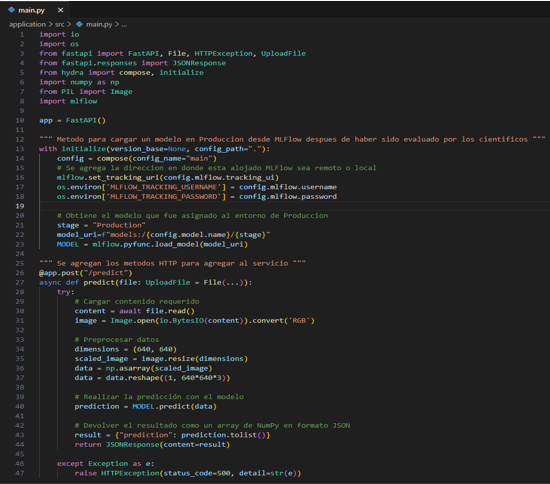
\includegraphics[width=1\textwidth]{resultados/codigoAPI.png}
\caption*{\footnotesize Fuente: Elaboración propia}
\label{fig:figuraCodigoAPI}
\end{figure}

Para la creación de aplicaciones web, se utiliza la herramienta Streamlit, una dependencia de Python que simplifica la creación de aplicaciones web interactivas diseñadas para la visualización de datos y prototipos\footnote{El código que genera la aplicación se encuentra en el siguiente enlace en GitHub \href{https://github.com/juferoto/mlops_project/tree/master/application/src/webapp}{aquí}}.

\newpage

\begin{figure}[h]
\centering
\caption{Estructura de la carpeta de la aplicación del proyecto}
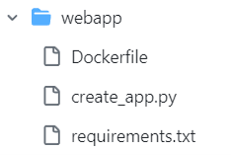
\includegraphics[width=0.4\textwidth]{resultados/estructuraCarpetaApp.png}
\caption*{\footnotesize Fuente: Elaboración propia}
\label{fig:figuraEstructuraCarpetaApp}
\end{figure}

Del contenido sobre el archivo Dockerfile se mencionara en el objetivo 4 y el archivo requirements.txt son las dependencias de Python que necesita la aplicación para funcionar.

\newpage

\begin{figure}[h]
\centering
\caption{Código del archivo create\_app.py para generar la aplicación}
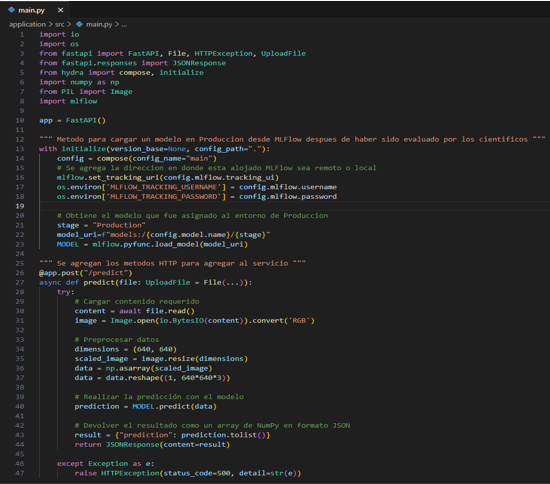
\includegraphics[width=0.8\textwidth]{resultados/codigoAPI.png}
\caption*{\footnotesize Fuente: Elaboración propia}
\label{fig:figuraCodigoAPI}
\end{figure}

Este es el código desarrollado para generar una aplicación destinada a ser consumida por los usuarios finales. Streamlit simplifica este proceso, ofreciendo una herramienta poderosa para desarrolladores que buscan crear rápidamente aplicaciones web interactivas, en este caso, enfocadas en datos.

Por otro lado, para iniciar MLFlow desde una máquina local, se utiliza el comando 
\begin{verbatim}
mlflow server
\end{verbatim}

Al ejecutar este comando desde la línea de comandos, se genera una dirección HTTP local que permite su uso y acceso directo desde el propio computador o servidor local\footnote{El video en donde se muestra el uso de MLFlow de manera local se encuentra \href{https://youtu.be/w4WX-OeOkrQ}{aquí}}.
Para hacer uso apropiado del MLFlow en local se debe cambiar el archivo de configuraciones ``main.yml'' del proyecto, colocando la dirección HTTP del MLFlow en local.

\begin{figure}[h]
\centering
\caption{Configuración local del MLFlow en el archivo ``main.yml''}
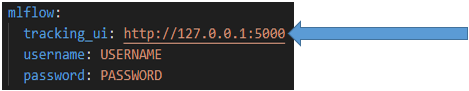
\includegraphics[width=1\textwidth]{resultados/cambioArchivoMain.png}
\caption*{\footnotesize Fuente: Elaboración propia}
\label{fig:figuraCambioArchivoMain}
\end{figure}

\subsubsection{Despliegue en entorno de pruebas}

Se procede con el despliegue del entorno de pruebas, y en este contexto, se presenta un video completo donde se reentrena el modelo de regresión logística, se lanza la aplicación y la API, y se demuestra el funcionamiento de la herramienta MLFlow, todo en un entorno local\footnote{El enlace al video completo en YouTube se encuentra adjunto \href{https://youtu.be/1rctGi8Sb7Q}{aquí}.}.

Para iniciar la API desde una máquina local, basta con ejecutar el siguiente comando: \begin{verbatim}python application\src\main.py\end{verbatim}

A su vez, para iniciar la aplicación desde una maquina local se debe ejecutar el siguiente comando: \begin{verbatim}streamlit run application\src\webapp\create_app.py\end{verbatim}

Además, también se deberá lanzar MLFlow utilizando el comando mencionado previamente. Los comandos empleados están detallados en el video para facilitar el despliegue del entorno de pruebas.